%Deep Learning
Deep learning architectures like belief networks and neural networks are accelerating the pace of innovation in various industries such as autonomous systems, 
retail shopping and social media. These complex computational models are used to churn large amounts of data so as to make predictions on new observations. 
For example, consider an autonomous vehicle driving through a busy street. The decision of stopping the vehicle will depend upon whether there is an 
impeding obstacle or a red signal. More importantly this decision will be needed to made in a small amount of time and may be based upon multiple noisy sensory inputs.
 
%CNNs
Convolutional Neural Networks (CNNs) have become extremely popular and being used to solve a variety of image recognition and computer vision tasks. 
More recent and advanced CNN architectures have become deeper and more complex having 10 to 20 
layers of Rectified Linear Units, hundreds of millions of weights, and billions of connections between units.
The reader is pointed to ~\cite{Bengio2009} for insights on deep architectures in general and ~\cite{DNNNature2015} for CNN-based learning and their recent advances.

While CNNs are an important thrust of research, they tend to be computationally expensive and deploying them on mobile platforms results in huge memory overheads. 
Another important insight recently unearthed by ~\cite{facenet}, is that the accuracies of CNNs can saturate after a few million images of training data.
Also the overall efficacy of the image recognition pipeline is contingent upon having a good region proposal scheme that feeds regions of interest (RoIs) into the CNN. 
Considering these challenges, a variety of strategies can be used to augment the capabilities of neural networks and we outline a few below.

\subsection{Visual Attention}
Humans process and respond to only certain streams of visual information depending upon the task at hand. 
From a systems perspective, visual attention can be used as an efficient mechanism to prioritize data processing.  
Pixel-level saliency models such as Attention by Information Maximization (AIM)~\cite{Bruceb} can be used in 
automatic household pantry organization and maintenance, particularly 
as part of assist systems for the visually impaired. Computationally, AIM determines visual salience based on the amount of information present in 
local regions of the image within the context of its surrounding region. 
Suppose a product (say cookies) is wrongly placed in a shelf that stores products of another type (say shampoo), the segment of the shelf image containing cookies is 
``less likely'' (higher self-information) to appear in the scene which mostly has image patches of shampoo, 
and therefore it is easily distinguishable or is considered ``salient''. This is shown in Figure~\ref{tab:saliencya}.
Once a salient region is detected, a second stage of object classification can be deployed to identify the wrongly placed object.  

%Saliency App 1
\begin{figure}[!htb]
\centering
\begin{tabular}{@{}l@{} @{}l@{}}
\vspace{-5pt}
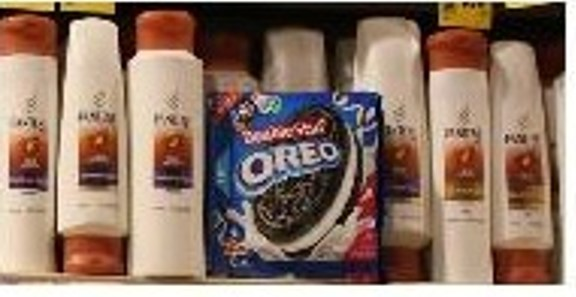
\includegraphics[width=0.5\linewidth,trim={0 0 0 0},clip]{mp1a.jpg} & 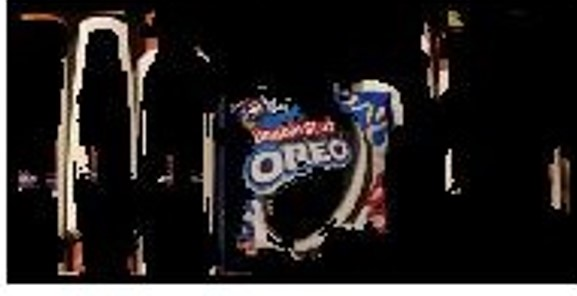
\includegraphics[width=0.5\linewidth,trim={0 0 0 0},clip]{mp1b.jpg}\\[\abovecaptionskip]
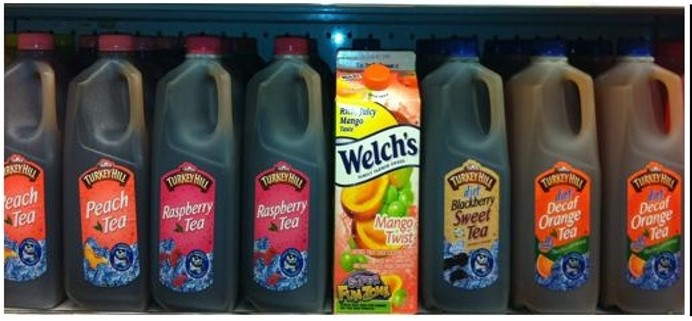
\includegraphics[width=0.5\linewidth,trim={0 0 0 0},clip]{mp2a.jpg} & 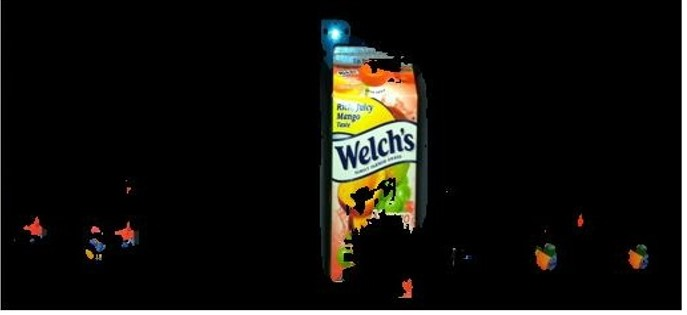
\includegraphics[width=0.5\linewidth,trim={0 0 0 0},clip]{mp2b.jpg}\\[\abovecaptionskip]
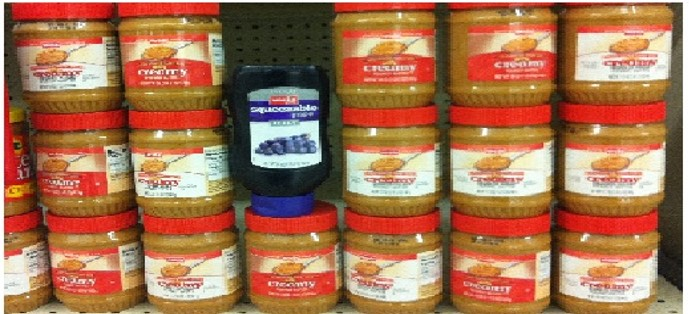
\includegraphics[width=0.5\linewidth,trim={0 0 0 0},clip]{mp3a.jpg} & 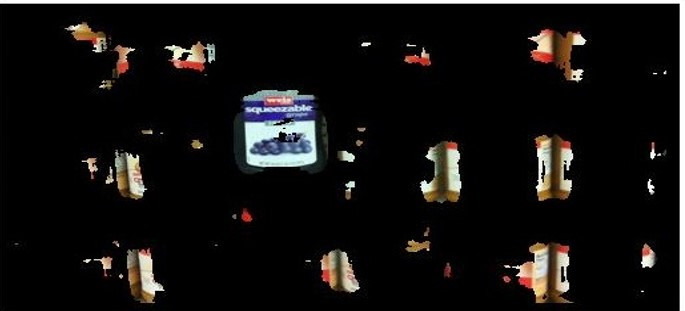
\includegraphics[width=0.5\linewidth,trim={0 0 0 0},clip]{mp3b.jpg}\\[\abovecaptionskip]
\small(a) Original image & \small (b) Thresholded saliency map\\
\end{tabular}
\caption{Saliency used for missplaced item detection.}
\label{tab:saliencya}
\end{figure}

Figure~\ref{tab:saliencyb} shows how a clustering of feature points
can intelligently segment items in a grocery shelf. Our approach works
well even with small and closely placed items of different types, as
are commonly seen in grocery environments.

%Saliency App 2
\begin{figure}[!htb]
\centering
\begin{tabular}{@{\hspace{1em}}l@{} @{\hspace{1em}}l@{}}
\vspace{-5pt}
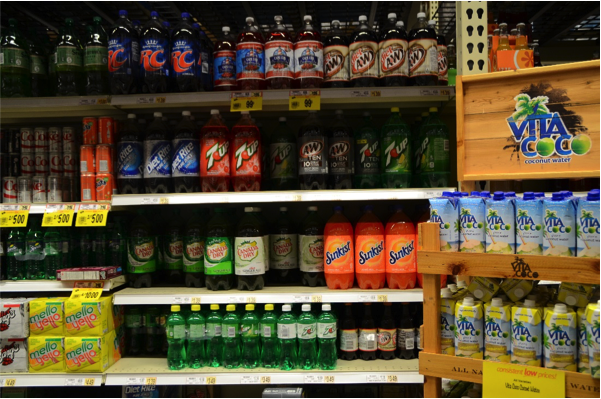
\includegraphics[width=0.45\linewidth,trim={0 0 0 0},clip]{surf_saliency_orig.png} & 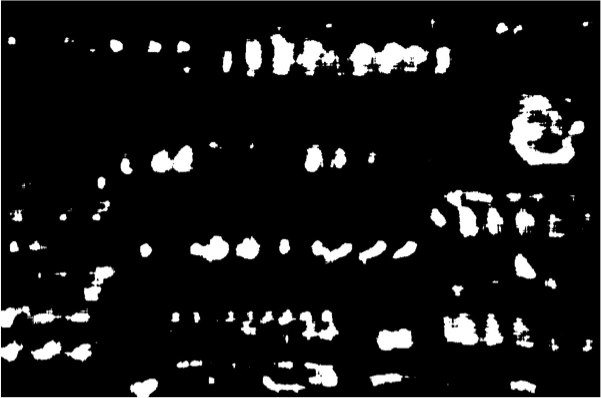
\includegraphics[width=0.45\linewidth,trim={0 0 0 0},clip]{surf_saliency.png}\\[\abovecaptionskip]
\small(a) Original image & \small (b) Segmented heatmap\\
\end{tabular}
\caption{SURF keypoint clustering used for product segmentation.}
\label{tab:saliencyb}
\end{figure}


At the other extreme, while grocery environments are diverse, in a
given grocery aisle there are often a lot of similar looking products
like cereal boxes, detergent bottles, etc. Rather than processing each
of these items as independent entities, we can localize similar RoIs,
run our classification engine on only one of them and then assign the
corresponding label to the entire group of similar
RoIs. Figure~\ref{tab:saliencyc} illustrates this flow where AIM is
used to generate initial seed RoIs that are then coupled with Speeded
Up Robust Features (SURF) keypoint matching to generate a list of RoIs
that are similar in structure.

%Saliency App 2
\begin{figure*}[!htb]
\centering
\begin{tabular}{@{}c@{} @{\hspace{1em}}c@{} @{\hspace{1em}}c@{}}
\vspace{-5pt}
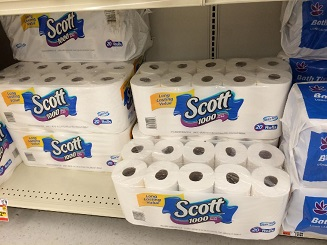
\includegraphics[width=0.31\linewidth,trim={0 0 0 0},clip]{scott_img.jpg} & 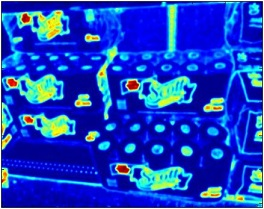
\includegraphics[width=0.30\linewidth,trim={0 0 0 0},clip]{scott_sali.jpg} & 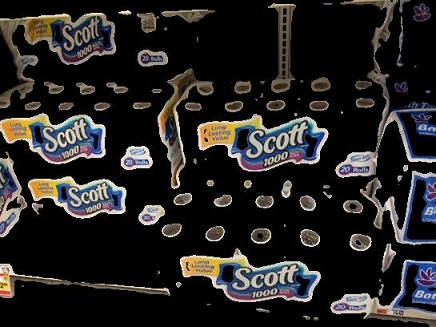
\includegraphics[width=0.31\linewidth,trim={0 0 0 0},clip]{scott_roi.jpg}\\[\abovecaptionskip]
\small(a) Original image & \small (b) Saliency Map & \small (c) Thresholded Map \\
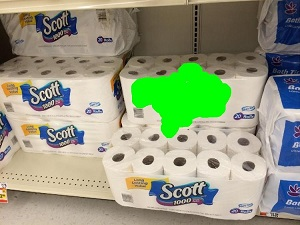
\includegraphics[width=0.31\linewidth,trim={0 0 0 0},clip]{scott_best_roi.jpg} & 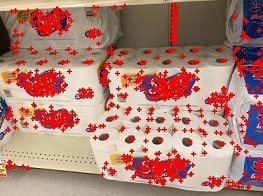
\includegraphics[width=0.30\linewidth,trim={0 0 0 0},clip]{scott_surf2.jpg} & 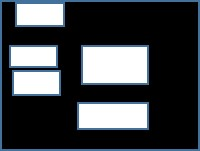
\includegraphics[width=0.31\linewidth,trim={0 0 0 0},clip]{scott_mask.jpg}\\[\abovecaptionskip]
\small(a) Best RoI & \small (b) SURF keypoints & \small (c) Regions of Interest \\
\end{tabular}
\caption{Saliency and SURF used to identify similar items.}
\label{tab:saliencyc}
\end{figure*}

\subsection{Context}
% Hierarchy of Parts
While deep learning models use learnt features to recognize objects in
a scene, visual systems can augment the current input data with
knowledge about the usual organization of the environment that can
provide greater scene context~\cite{estimedia2015} and heirarchical
models~\cite{hop} that can reason about objects as collections of
parts.  Compositional rules can be used to build context cues to
recognize objects never seen before if they contain previously seen
sub-pieces. For example, if a product's packaging changes or displays
a seasonal advertisement, but key portions of the branding remain,
then the product could still be recognized even if this version has
never previously been seen.  Similarly, when it comes to recognizing
objects in video streams, spatial and temporal context can play a huge
role in reducing the workload on computationally intensive models such
as CNNs.  For example, in~\cite{estimedia2015}, the authors proposed a
Bayesian network called the Visual Co-occurrence Network (ViCoNet)
where objects were represented as nodes and edges represented spatial
relations between them. Figure~\ref{fig:viconet} shows an example of a
subgraph in such a system, which could very well represent a
fresh-fruit section of a grocery shop. From this graph, it can be seen
that, if the previous classification is a peach, then the next region
is more likely a plum rather than mango, and this probability can
be used to bias the classifications. Moreover, this graph naturally
encodes aisle relationships, and can be used to feed an aisle
predictor to narrow the set of plausible classes for any
identification. These pruning features allowed the system using this
network to improve performance as well as recognition rates.

\begin{figure}[!htb]
\centering
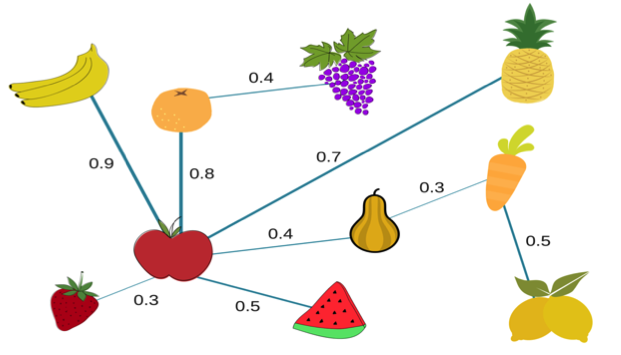
\includegraphics[width=0.9\linewidth]{viconetexample.png}
\caption{Spatial relations exist between frequently co-occurring objects. These relationships can then be used as context cues to guide the recognition task.}
\label{fig:viconet}
\end{figure} 

\subsection{Multimodal Fusion}
Humans use multisensory information from different sensory systems and combine it to influence 
perception, decisions, and overt behavior~\cite{stein2009neural}. Wearables can be used in a similar fashion to help users in different tasks. 
A rich topic of exploration is figuring out a way to fuse multi-sensor information, especially data from vision that is fundamentally two-dimensional with a temporal 
unidimensional stream of data from other sensors to make predictions of the current state of the user. Multi-sensor information coming in from different devices can be 
streamed to distributed networks that can then make real-time updates. In Figure~\ref{tab:sensor}, we illustrate data recorded from a wearable device while two users
walk in three different directions. As can be seen, these sensors are sensitive enough to be used as localization cues. 

%MultiModal Analysis
\begin{figure*}[!htb]
\centering
\begin{tabular}{@{}c@{} @{}c@{} @{}c@{}}
\vspace{-5pt}
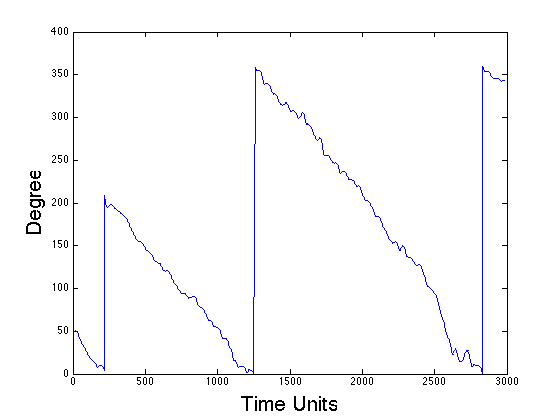
\includegraphics[width=0.33\linewidth,trim={25 5 30 5},clip]{walk_left_p1.png} & 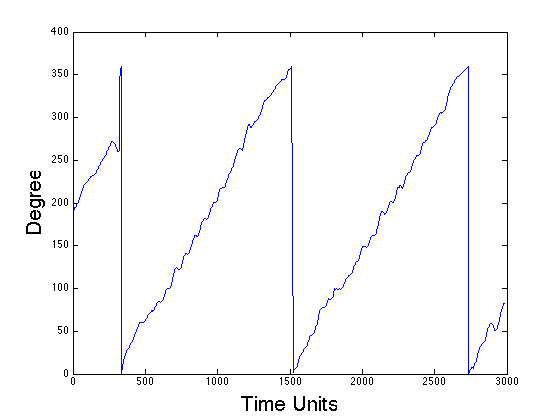
\includegraphics[width=0.33\linewidth,trim={25 5 30 5},clip]{walk_right_p1.png} & 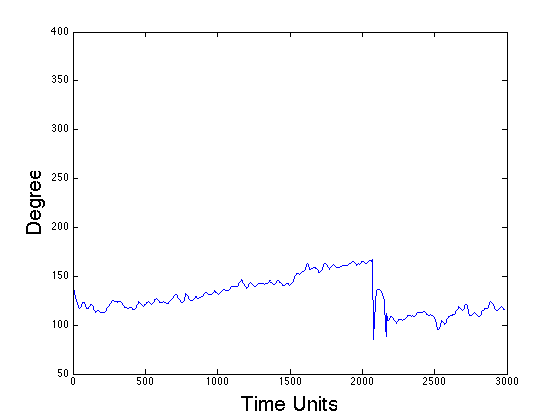
\includegraphics[width=0.33\linewidth,trim={25 5 30 5},clip]{walk_straight_p1.png}\\[\abovecaptionskip]
\small(a) Person 1 - Left & \small (b) Person 1 - Right & \small (c) Person 1 - Straight\\
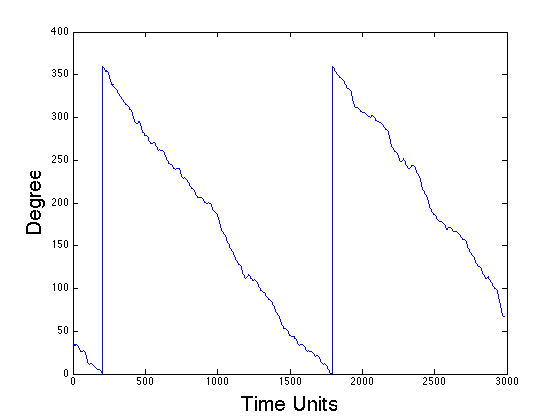
\includegraphics[width=0.33\linewidth,trim={25 5 30 5},clip]{walk_left_p2.png} & 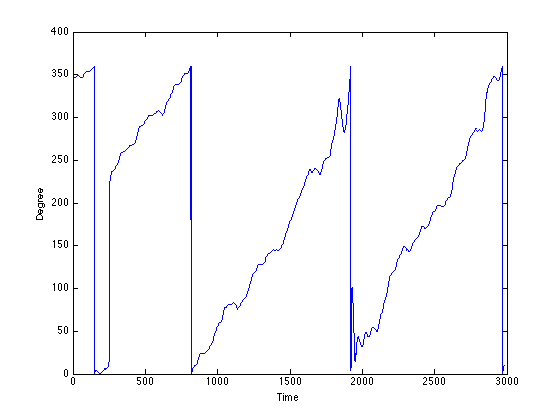
\includegraphics[width=0.33\linewidth,trim={25 5 30 5},clip]{walk_right_p2.png} & 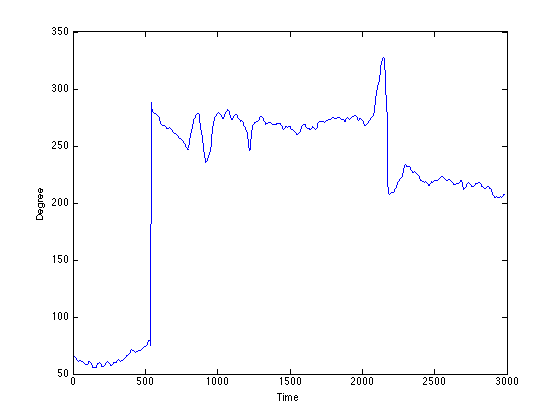
\includegraphics[width=0.33\linewidth,trim={25 5 30 5},clip]{walk_straight_p2.png}\\[\abovecaptionskip]
\small(a) Person 2 - Left & \small (b) Person 2 - Right & \small (c) Person 2 - Straight\\
%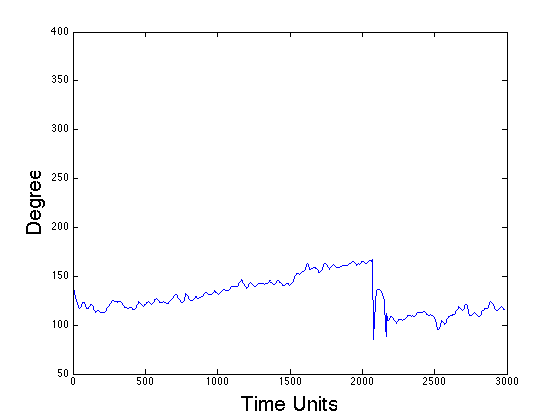
\includegraphics[width=0.5\linewidth,trim={0 0 0 0},clip]{walk_straight_p1.png} & 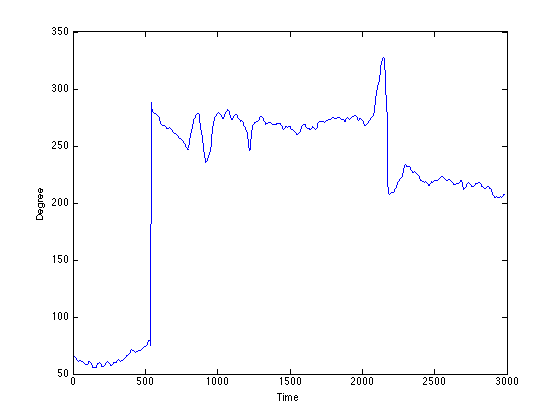
\includegraphics[width=0.5\linewidth,trim={0 0 0 0},clip]{walk_straight_p2.png}\\[\abovecaptionskip]
%\small(a) Person 1 - Straight & \small (b) Person 2 - Straight\\
\end{tabular}
\caption{Temporal sensor information used for localization.}
\label{tab:sensor}
\end{figure*}

In the next section, we move further down the stack and discuss relevant system-level design and architectures that can further enhance the performance of mobile 
visual-assist systems. 
